\scanpage{3}
% archive foliation: 2
\[
H_A^{\deleted{\unsure{*}}}
\bigl(f^*(\underset{\substack{\vert\\b^\circ}}{\Psi_*}),
\underset{\substack{\vert\\a^\circ}}{\Phi^{\unsure{*|\circ}}}\bigr)
\overset{?}{\simeq}
H_B\bigl(\Psi_*,f^\circ_!(\Phi^*)\bigr)
\]
\[
\operatorname{Hom}_B(b,f(a))=
\operatorname{Hom}_{\widehat B}(b,f_{\unsure{!}}(a))
\overset{?}{\simeq}\operatorname{Hom}_{\widehat A}(\unsure{f^*b},a)
\]
\[
H_A\bigl(\underset{\wedge}{f^*(b)},\underset{\substack{\vert\\\vee}}a\bigr)
\simeq H_B\bigl(\underset{\wedge}{b},\underset{\vee}{f^\circ(a)}\bigr)
=\operatorname{Hom}_B(b,f(a))
\]
\[
\unsure{\Vert}\quad\inserted{\overset{\wedge\quad\vee}{\operatorname{Hom}}}
\quad\deleted{\operatorname{Hom}_{\widehat A}(f^*(b),a)=\operatorname{Hom}}
\]
\[
f^*(b)=\varinjlim_{a'\text{ ds }A/b}a'^{\unsure{\circ}}
\]
\[
\unsure{\forall|H_A}\ \varprojlim_{a'\text{ ds }A/b}\operatorname{Hom}_A(a',a)
\]

% The following draft is written in the opposite orientation and crossed by two long diagonal strokes.
\diagram{\begin{array}{l}
\deleted{\widehat B^\circ\unsure{\longrightarrow|{-}}\widehat A}\quad
\left\{\deleted{\unsure{B\times}}\ \deleted{\widehat B^\circ\times}\right.\\
\deleted{B^\vee\unsure{\longrightarrow|{-}}\widehat A}\\
\deleted{\widehat A^\circ\unsure{\longrightarrow|{-}}\widehat B}\\
\deleted{A^\vee\unsure{\longrightarrow|{-}}\widehat B}
\end{array}}

\figure{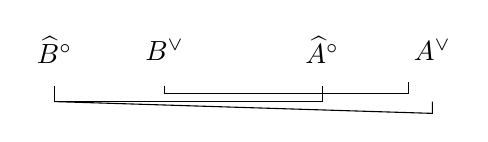
\begin{tikzpicture}[x=1cm,y=1cm]
\node at (0,1) {$\deleted{\widehat B^\circ}$};
\node at (1.4,1) {$\deleted{B^\vee}$};
\node at (3.4,1) {$\deleted{\widehat A^{\unsure{\circ}}}$};
\node at (4.8,1) {$\deleted{A^\vee}$};
\draw (0,.55)--(0,.35)--(3.4,.35)--(3.4,.55);
\draw (1.4,.55)--(1.4,.45)--(4.5,.45)--(4.5,.6);
\draw (0,.35)--(4.8,.2)--(4.8,.35);
\end{tikzpicture}}

\diagram{\begin{array}{c|c}
\deleted{\widehat A^\circ}&\deleted{\widehat B^\circ}\\
\deleted{A^\vee}&\deleted{B^\vee}
\end{array}}

\diagram{\begin{tikzcd}[column sep=large,row sep=small]
\deleted{\widehat B^\circ}\arrow[r,"\deleted{!}"] & \deleted{\widehat A}
& \deleted{\widehat B^\circ\times\widehat A^\circ}\arrow[r,"\deleted{!!}"]
& \deleted{\operatorname{Ens}}\arrow[dddd,no head,bend left=20]\\
&&\deleted{\widehat B^\circ\times A^\vee}\arrow[r,"\deleted{!}","\deleted{!}"']
&\deleted{\operatorname{Ens}}\arrow[ddddd,no head,bend left=48]\\
\deleted{B^\vee}\arrow[r,"\deleted{!}"'] &\deleted{\widehat A}
&\deleted{B^\vee\times\widehat A^\circ}\arrow[r,"\deleted{!}","\deleted{!}"']
&\deleted{\operatorname{Ens}}\arrow[ddd,no head,bend left=35]\\
&&\deleted{B^\vee\times A^\vee}\arrow[r,"\deleted{!!}"']
&\deleted{\operatorname{Ens}}\arrow[dddd,no head,bend left=65]\\
\deleted{\widehat A^\circ}\arrow[r,"\deleted{!}"] &\deleted{\widehat B}
&\deleted{\widehat A^\circ\times\widehat B^\circ}\arrow[r,"\deleted{!!}"]
&\deleted{\operatorname{Ens}}\\
&&\deleted{\widehat A^\circ\times B^\vee}\arrow[r,"\deleted{!}","\deleted{!}"']
&\deleted{\operatorname{Ens}}\\
\deleted{A^\vee}\arrow[r,"\deleted{!}"'] &\deleted{\widehat B}
&\deleted{A^\vee\times\widehat B^\circ}\arrow[r,"\deleted{!}","\deleted{!}"']
&\deleted{\operatorname{Ens}}\\
&&\deleted{A^\vee\times B^\vee}\arrow[r,"\deleted{!!}"']
&\deleted{\operatorname{Ens}}
\end{tikzcd}}
\figure{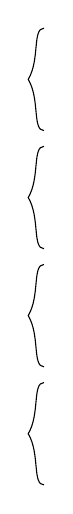
\begin{tikzpicture}
\foreach \y in {0,1.5,3,4.5}{\draw (0,\y+.65) .. controls (-.15,\y+.65) and (-.05,\y+.25) .. (-.2,\y)
 .. controls (-.05,\y-.25) and (-.15,\y-.65) .. (0,\y-.65);}
\end{tikzpicture}}

\margin{\deleted{$\underline{\operatorname{Hom}}(\widehat A^\circ,\unsure{''})$}}
\margin{\deleted{\uuline{Hom}\unsure{.}}}
\diagram{\begin{array}{l|ll}
&\deleted{\widehat A}\ \deleted{\text{contr}}&\deleted{\text{contr }\widehat B}\\
&\deleted{A^\vee}\ \deleted{\text{co}}&\deleted{B}
\end{array}}

\diagram{\begin{tikzcd}[column sep=small,row sep=small]
&&{}&&&&{}\\
{}&\deleted{\widehat A^\circ-\widehat B}\arrow[ddl,no head]\arrow[dr,no head]
&&\deleted{\widehat B^\circ-\widehat A}\arrow[dl,no head]\arrow[drrr,no head]&{}&&\\
&&\deleted{\widehat A,\widehat B}\arrow[uu,no head]\arrow[dll,no head,"\deleted{\widehat A}"']
\arrow[rrrr,no head,"\deleted{\widehat B}"]&&&&\deleted{A^\vee,\widehat B}\arrow[uu,no head]\arrow[dll,no head,"\deleted{A^\vee}"]\\
\deleted{\widehat A,B^\vee}\arrow[uu,no head]\arrow[rrrr,no head,"\deleted{B^\vee}"']&&&&\deleted{A^\vee,B^\vee}\arrow[uu,no head]&&
\end{tikzcd}}

\figure{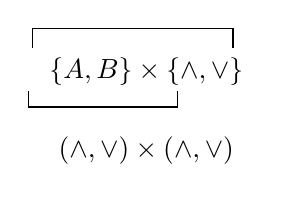
\begin{tikzpicture}[x=1cm,y=1cm]
\node at (1.6,1) {$\deleted{\{A,B\}\times\{\wedge,\vee\}}$};
\node at (1.6,0) {$\deleted{(\unsure{\wedge},\vee)\times(\wedge,\vee)}$};
\draw (.15,1.3)--(.15,1.55)--(2.7,1.55)--(2.7,1.3);
\draw (.1,.75)--(.1,.55)--(2,.55)--(2,.75);
\end{tikzpicture}}

\diagram{\begin{tikzcd}[column sep=small,row sep=large]
&&\deleted{\underline{\operatorname{Hom}}^!(\widehat A^\circ,\widehat B)}\arrow[dll,bend right=20]\arrow[drr,bend left=15]&&\\
\deleted{\underline{\operatorname{Hom}}^{\unsure{!!}}_{\deleted{\unsure{!}}}(\widehat A^\circ,\widehat B^\circ;\operatorname{Ens})}
&&\deleted{\widehat A}\arrow[dd,no head]
&&\deleted{\underline{\operatorname{Hom}}^{\unsure{!}}_{!}(\widehat A^\circ,B^\vee;\operatorname{Ens})}\\
&\deleted{\wedge\wedge}\ \deleted{\unsure{\operatorname{Ens}\ \underline{\operatorname{Hom}}}}
&&\deleted{\wedge\vee}&\unsure{\wr}\arrow[d,no head]\\
\deleted{\underline{\operatorname{Hom}}^!(\widehat B^\circ,\widehat A)}\arrow[uu,bend left=10]\arrow[ddd,bend right=15]
&\deleted{\widehat B}\arrow[r,no head]
&\deleted{\widehat{(A\times B)}}\arrow[r,no head]
&\deleted{B^\vee}
&\deleted{\underline{\operatorname{Hom}}_!(B^\vee,\widehat A)}\arrow[uu,bend right=20]\arrow[ddd,bend left=15]\\
&\deleted{\vee\wedge}
&\deleted{A^\vee}\arrow[u,no head]
&\deleted{\vee\vee}\ \deleted{\unsure{\underline{\operatorname{Hom}}}}&\\
&&&&\\
\deleted{\underline{\operatorname{Hom}}^{\unsure{!}}_{\unsure{!}}(\unsure{A^\vee},\unsure{\widehat B^\circ};\operatorname{Ens})}
&&\deleted{\underline{\operatorname{Hom}}_!(A^\vee,\widehat B)}\arrow[ll]\arrow[rr,bend right=15]
&&\deleted{\underline{\operatorname{Hom}}_{!!}(A^\vee,B^\vee;\operatorname{Ens})}\\
\deleted{\unsure{(\widehat A,\widehat B,\operatorname{Ens})}}&&&&
\end{tikzcd}}

\figure{\begin{tikzpicture}[x=1cm,y=1cm]
\draw (0,5.7)--(12,0.1);
\draw (5.8,0)--(11.7,7.2);
\end{tikzpicture}}

\diagram{\begin{array}{l}
\texttt{//\unsure{PREDONMA|PREDONAA} JOB CNU0049\$NODER=PREDONT} \\
\texttt{/*JOBPARM L=15} \\
\texttt{//COMP EXEC FORTXC,PARM=TERM,REGION=300K} \\
\texttt{//FORT.SYSPRINT DD DSN=\&MESSYS,SPACE=(CYL,4),UNIT=SYSDA,DISP=(MOD,PASS)} \\
\texttt{//FORT.SYSTERM DD DSN=\&MESCOM,SPACE=(CYL,2),UNIT=SYSDA,DISP=(MOD,PASS)} \\
\texttt{//SYSIN DD DSN=CNU1.MODULEF.V33.INTERME1(MEFCONVS),DISP=OLD} \\
\texttt{//CUTR EXEC PGM=CUTTER} \\
\texttt{//STEPLIB DD DSN=CNU2.MODULEF.UTIA,DISP=SHR} \\
\texttt{//TERMINAL DD DSN=\&MESCOM,DISP=(OLD,DELETE)} \\
\texttt{//OBJECT1 DD DSN=\&ORJ,DISP=(OLD,DELETE)} \\
\texttt{//SOURCE1 DD DSN=\&MESSYS,DISP=(OLD,DELETE)} \\
\texttt{//SYSPRINT DD DUMMY} \\
\texttt{//SOURCE2 DD DSN=\&SOURCE,SPACE=(CYL,4),UNIT=SYSDA,DISP=(MOD,PASS)} \\
\texttt{//OBJECT2 DD DSN=\&ORJ2,SPACE=(CYL,3),UNIT=SYSDA,DISP=(MOD,PASS)} \\
\texttt{//UPDT EXEC PGM=UPDATE,COND=(0,NE,CUTR),PARM=NEW} \\
\texttt{//STEPLIB DD DSN=CNU2.MODULEF.UTIA,DISP=SHR} \\
\texttt{//SYSIN DD DSN=\&SOURCE,DISP=(OLD,DELETE)} \\
\texttt{//SYSIN2 DD UNIT=SYSDA,SPACE=(CYL,4)} \\
\texttt{//SYSUT\deleted{\unsure{1}}\inserted{2} DD DSN=CNU2.MODULEF.CONVS,DISP=(,CATLG),SPACE=(TRK,(20,2,35)),} \\
\texttt{// DCB=(RECFM=FB,LRECL=80,BLKSIZE=19040),UNIT=SYSDA,VOL=SER=SYSPPP} \\
\texttt{//SYSPRINT DD SYSOUT=*} \\
\texttt{//LIEN EXEC FORTXL,COND=(0,NE,CUTR)} \\
\texttt{//LKED.SYSLIN DD DSN=\&ORJ2,DISP=(OLD,DELETE)} \\
\texttt{//LKED.SYSLMOD DD DSN=CNU2.MODULEF.CONV,SPACE=(TRK,(40,4,35)),} \\
\texttt{// DCB=(RECFM=U,BLKSIZE=19040),UNIT=SYSDA,VOL=SER=SYSPPP,DISP=(,CATLG)} \\
\texttt{//FIN EXEC PGM=IEFBR14,COND=((0,EQ,UPDT),(4,GE,LIEN.LKED),EVEN)} \\
\texttt{//SOURCE DD DSN=CNU2.MODULEF.CONVS,DISP=(OLD,DELETE)} \\
\texttt{//MODEX DD DSN=CNU2.MODULEF.CONV,DISP=(OLD,DELETE)} \\
\texttt{//}
\end{array}}

\figure{\begin{tikzpicture}[x=1cm,y=1cm]
\draw[->](0,4.7)--(.5,4.7);
\draw[->](0,2.2)--(.5,2.2);
\draw[->](0,1.2)--(.5,1.2);
\draw[->](0,.8)--(.5,.8);
\draw[->](6.5,2.2)--(6,2.2);
\end{tikzpicture}}
